% !TEX root = Installation.tex

\chapter{Installation / Konfiguration} \label{def:installation}
Damit beide Frameworks miteinander verglichen werden k�nnen, muss zun�chst Cypress installiert werden. Die bestehende Selenium-Pytest Infrastruktur existiert bereits im Unternehmen und muss nur mithilfe des Versionsverwaltungstools Git, heruntergeladen werden. 
\newline\newline
In diesem Kapitel wird beschrieben, wie die Installation und Konfiguration von Cypress stattfindet. Zus�tzlich werden die Voraussetzungen zur Installation von Cypress erl�utert und welches System zur Testautomatisierung im Rahmen dieser Arbeit verwendet wird.

\section{Umgebung}
Das Unternehmen glomex ben�tigt ein System, dass alle Anforderungen unterst�tzt. Die Umgebung muss von Cypress.io sowie von Selenium unterst�tzt werden. 
\newline\newline
Cypress wird derzeit (Stand 13.02.2018) auf folgenden Plattformen supportet \autocite{cypress}:
\begin{itemize}
	\item Mac OS 10.9+ (Mavericks+), only 64bit binaries are provided for macOS.
	\item Linux Ubuntu 12.04+, Fedora 21, Debian 8.
	\item Windows 7+, only 32bit binaries are provided for Windows.
\end{itemize}

Selenium setzt nur einen installierten Browser und eine der folgenden Programmiersprachen voraus \autocite{selenium}:
\begin{itemize}
	\item Java
	\item C\# 
	\item Ruby
	\item Python
	\item Javascript (Node)
\end{itemize}

Da unternehmensweit bei der glomex Mac OS genutzt wird und beide Frameworks, sowohl Cypress als auch Selenium unterst�tzt werden, wurde entschieden Mac OS zu verwenden. 

\section{Cypress Test Runner} \label{def:cypress_test_runner}
\subsection{Installation unter Mac OS}

\begin{figure}[H]
	\centering
	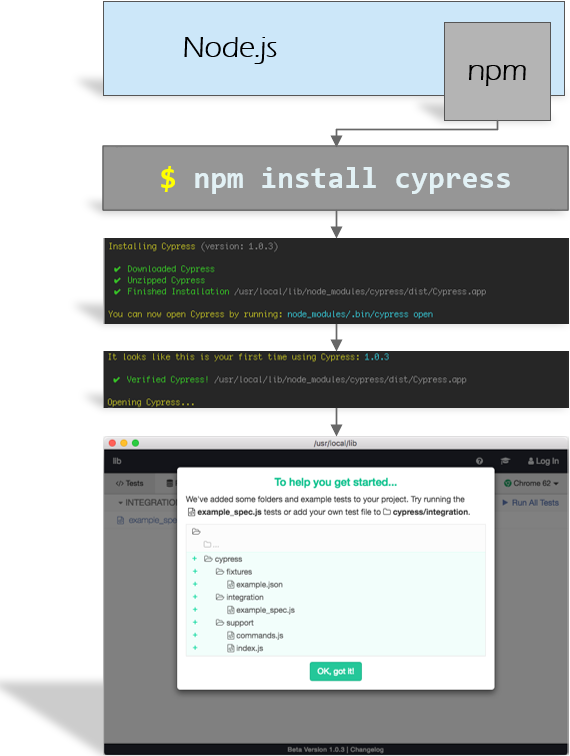
\includegraphics[width=0.98\textwidth]{06_Bilder/cypress_installationsprozess.png}
	\setlength{\abovecaptionskip}{1em}
	\caption{Cypress Installationsprozess (Mac OS)}
	\label{img:cypress_install_grafik}
\end{figure}

Bei der Verwendung von Mac OS muss erst das Programm \enquote{Node.js} installiert werden, da dieses den \gls{packagemanager} Npm enth�lt (siehe Abbildung \ref{img:cypress_install_grafik}). Npm ist ein \gls{packagemanager} f�r JavaScript und enth�lt tausende frei zum Download verf�gbare Pakete \autocite{npm}. F�r das Betriebssystem Mac OS wird empfohlen, Cypress mithilfe von Npm zu installieren, da Npm in der Lage ist, Cypress zu aktualisieren und zu installieren \autocite{cypress}.  
\newline\newline
Nach der Installation steht der Befehl \enquote{npm} in einer eingabebasierenden Benutzerschnittstelle der sogenannten \gls{bash} zur Verf�gung. Mithilfe des Befehls \enquote{npm install cypress} kann nun die Installation des Cypress Test Runners gestartet werden (siehe Abbildung \ref{img:cypress_install_grafik}). 

\subsection{Konfiguration} \label{def:konfiguration}
Nach Abschluss der Installation ist der sogenannte \enquote{Cypress Test Runner} installiert. Dieser enth�lt alle wichtigen Tools und Einstellungen um Tests zu starten und Ergebnisse auszuwerten.
\newline\newline
Es gibt zwei Wege den Cypress Test Runner zu starten:

\begin{itemize}
	\item \textbf{Mithilfe des \gls{bash}befehls \enquote{node\_modules/.bin/cypress open} (siehe Abbildung \ref{img:cypress_install_grafik})}\\
	Dabei ist zu beachten, dass der Befehl nur funktioniert, wenn der Anwender sich im Cypress Projektverzeichnis befindet. Zus�tzlich ist der Anwender mit dieser Methode nicht in der Lage das Projektverzeichnis auszuw�hlen.
	\item \textbf{Direkt �ber Programme}\\
	Bei dieser Methode kann der Anwender selber ein vorhandenes Projektverzeichnis ausw�hlen oder ein neues erstellen.

\end{itemize}

\subsection{Update} \label{def:cypress_update}
Cypress �berpr�ft vor jedem Start ob eine neue Version verf�gbar ist. Sobald eine neue Version zur Verf�gung steht, erscheint ein Update-Button im unteren Bereich des Cypress Test Runners. �ber diesen Button wird einem explizit angezeigt, welche Schritte der Anwender zu gehen hat, damit Cypress aktualisiert wird. 

\begin{figure}[H]
	\centering
	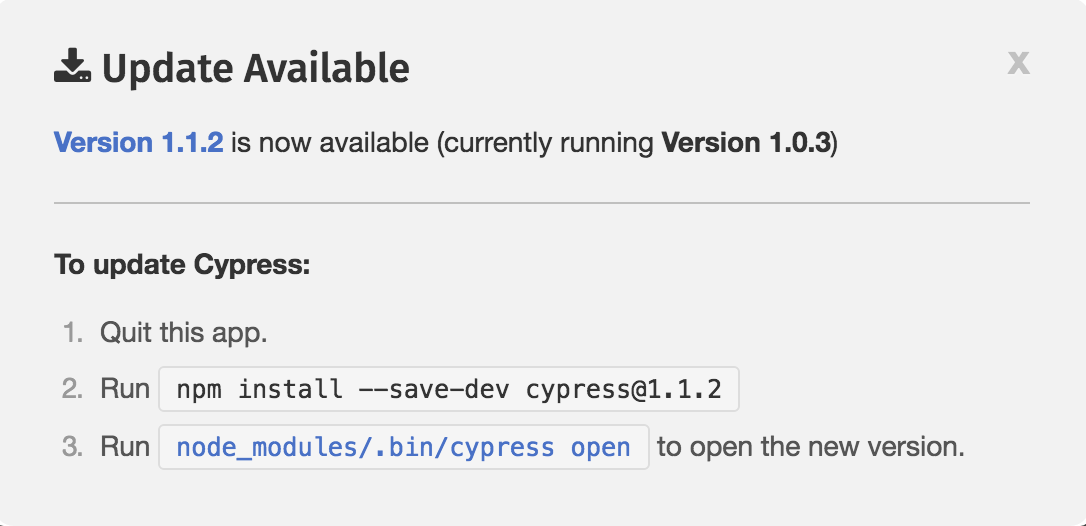
\includegraphics[width=1.0\textwidth]{06_Bilder/cypress_update.png}
	\setlength{\abovecaptionskip}{0em}
	\caption{Cypress Update}
	\label{img:cypress_update}
\end{figure}

Nachdem das Update durchgef�hrt wurde, kann die neue Version des Cypress Test Runners, wie in Kapitel \ref{def:konfiguration} beschrieben, gestartet werden.

\section{Visual Studio Code} \label{def:visual_studio}
Sobald der Cypress Test Runner installiert wurde, wird noch zus�tzlich ein Editor zum Erstellen und Editieren der Tests in Form von JavaScript (.js) Dateien ben�tigt. Im Rahmen dieser Arbeit wurde entschieden \enquote{Visual Studio Code} zu verwenden, da dieser Editor alle g�ngigen Plattformen unterst�tzt und ein \gls{syntax} f�r JavaScript beinhaltet. Im Vergleich zur Installation des Cypress Test Runners, muss nur eine Installationsdatei heruntergeladen und installiert werden \autocite{visualstudio}. 